\chapter{Analysis Of Existing}

As said before, drone swarm are governed by these models mobility. Our study of the existing is therefore divided into several parts.

\section{Summary of the problem}

The issue of this paper is to scan an area as efficiently as possible and as quickly as possible, at least once per hour. This area will be scanned by a UAV swarm that will cooperate and communicate each other.

\section{Existing models}

Many mobility models exist with different characteristics. All these models are used to define movements for swarm of UAV. Most models are based on real-life situations such as road maps, or on the behavior of many animals (ants, birds, termites, wolves etc). We will expose some of them we consider the most important and most interesting for our case.

\subsection{Random Walk}

First described by Einstein in 1926, it was developed to mimic the extremely unpredictable movement of many entities in nature. An mobility node (MN) moves from its position to a new one by randomly choosing a direction and speed chosen by pre-defined ranges, [speedmin, speedmax] and [0, 2PI]. At the end of a constant time interval t or a constant distance traveled d, a new speed and direction are calculated. If a MN during his travel reaches a simulation boundary, it « bounces » off the simulation border with an angle determined by the incoming direction and continues to this new path.
It's a memory-less mobility pattern because it retains no knowledge of its old locations and speed values. Therefore, the current position and speed of a MN is independent of its past location and speed. This can generate unrealistic movement because of sudden stops and sharp turns. If the specified time or distance of a MN motion is short, the resulting movement pattern will be a random roaming pattern restricted to a small part of the simulation area. The Figure \ref{RandomWalk} shows an example of the movement observed from this model. All the MN begin in the center of the 300mx600m simulation area (at the position (150,300)). Every 60 seconds, each MN randomly choose a direction between 0 and 2PI, and a speed between 0 and 10m/s.

\begin{figure}[h]
\center
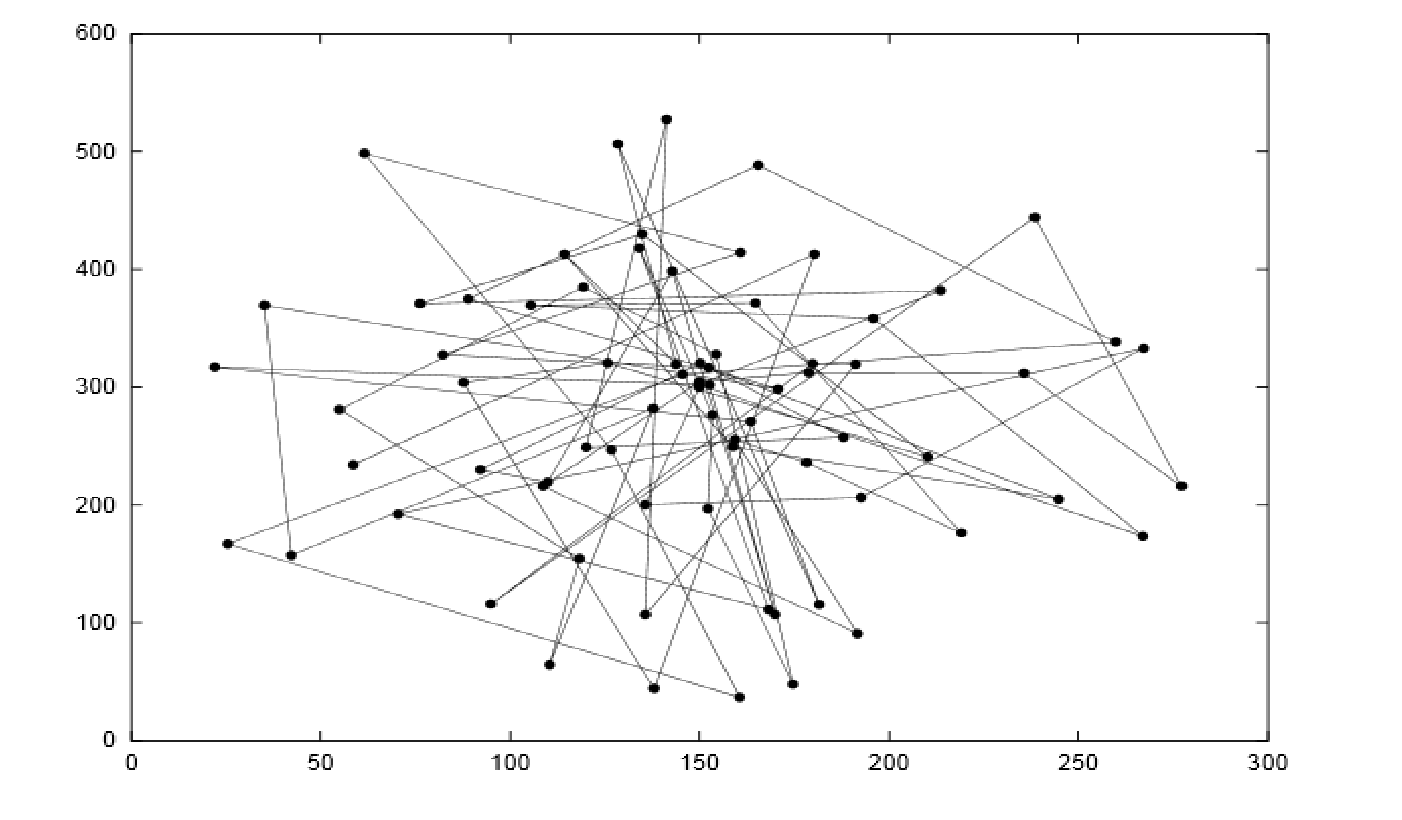
\includegraphics[width=7cm,height=50mm]{../images/randomwalk1.png}
\caption{\label{RandomWalkFig}Resulting pattern of a MN using the Random Walk Mobility Model}
\end{figure}



\subsection{Random Waypoint}

Includes pause times between changes in direction and/or speed.Once this time expires, the MN chooses a random destination and a speed, that is uniformly distributed between [minspeed, maxspeed]. The movement pattern of a MN who uses the RWaypointMM is similar to the RWalkMM if pause time is zero and [minspeed, maxspeed] = [speedmin, speedmax]. The Figure \ref{RandomWaypointFig} shows an example of the resulting pattern from the Random Waypoint Mobility Model.

\begin{figure}[h]
\center
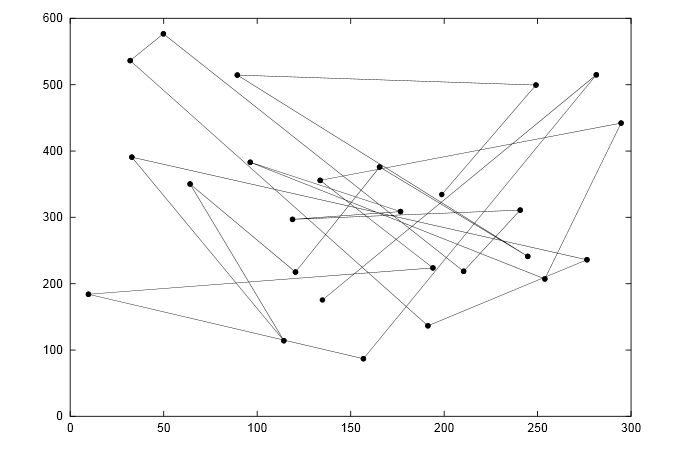
\includegraphics[width=7cm,height=50mm]{../images/randomwaypoint1.png}
\caption{\label{RandomWaypointFig}Resulting pattern of a MN using the Random Waypoint Mobility Model}
\end{figure}

During a run, MNs are initially distributed randomly around the simulation area. Figure \ref{RandomWaypointFig2} shows the average MN neighbors percentage of the MNs. The average is the cumulative percentage of total MNs that are a given MN's neighbor. Therefore, if the network have 20 node and a node has 2 neighbors, then the node's current neighbors percentage is 10\%. Moreover, during the first 600 seconds, due to initially distributed randomly of the MNs around the simulation area, there is an high variability in the average MN neighbors percentage.
In the paper, there is presented three possible solutions to avoid this initialization problem. The first is to save the location of the MNs after the initial high variability and use this position as the initial starting point of the MNs in the next simulations. Second is to change the initial distribution of the MNs in a specific area to be a distribution more common the model, like for example, initially placing the MNs in a triangle distribution. Lastly, the beginning of each simulation produce initialization problem due to the random distribution of the MNs around the simulation area. Throw out the initial 1000 seconds of simulation time in each simulation ensure that the initialization problem is removed even if the MNs move slowly. But if the MNs move fastly, we can discard fewer seconds of simulation time. This third solution ensures that each simulation has a random initial configuration.

\begin{figure}[h]
\center
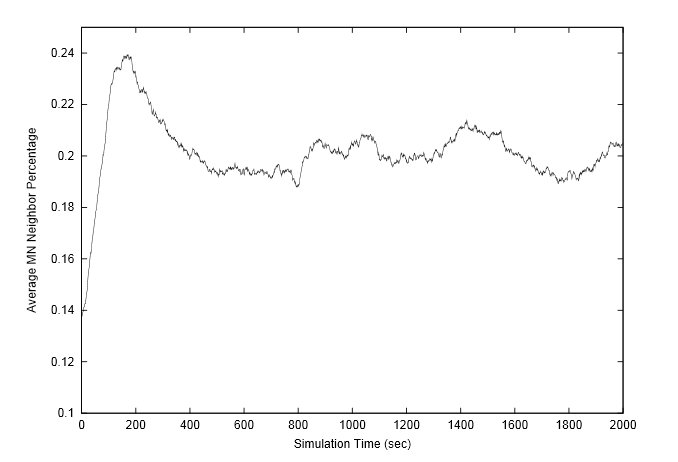
\includegraphics[width=7cm,height=50mm]{../images/randomwaypoint2.png}
\caption{\label{RandomWaypointFig2}Average neighbor percentage vs. time}
\end{figure}


\subsection{City section}

The aim of this model is to propose a realistic model. It bases on the vehicle's movement on road maps. The specificity of this model is the map depends on each geographical zone. Here, vehicles are mobile nodes.\\\\

The mapping data blocks are available from the office Americans of the census. The map information is retrieved from text files. These files are composed of several elements:

\begin{itemize}
\item The unique identifier for a specified road.
\item The nature of the road: it can be a highway or a street.
\item The longitude of the start of position.
\item The latitude of the start of departure
\item The latitude of arrived.
\item The longitude of arrived.
\end{itemize}

All the intersections of the map are represented by nodes not mobile.
This model also considers the volume of traffic : more traffic, the more the line representing the road will be thick.
This model is also sensitive at the speed of cars (depending in particular on the hour). For example, we can consider that the speed of vehicular traffic in the morning is much smaller than at the beginning of the afternoon.\\\\

Here is the progress of this model. Every node begins in a point chosen randomly and its destination is chosen also randomly. The strategy of every node is to look for the shortest way until the destination. To achieve it, the algorithm of Dijkstra is used. Several parameters has to be considered in this algorithm as the speed or the traffic. This route can be dynamically changed. When a node reaches its destination, it begins again all the process described previously. Concerning the node's speed, it is limited to more or less 5\% of the speed registered in the file.\\
For example, here is a representation of the model. We see here that the traffic is little sparse, but with very different speeds. The comparisons of these two regions base themselves on the inaccessible pairs, the length of the average route and to finish the changes of neighbors.\\

This article proposes two situations.
The first situation, which they call region A, proposes a very dense road network with a constant speed limit on all the road network. The second situation, which they call region B, proposes a road network much less dense than the precedent, but with different speeds of movements.

The comparisons of these two regions base themselves on the inaccessible pairs, the length of the average route and to finish the changes of neighbors.\\

Here are representations of these two regions.\\\\

\begin{tabular}{cc}
   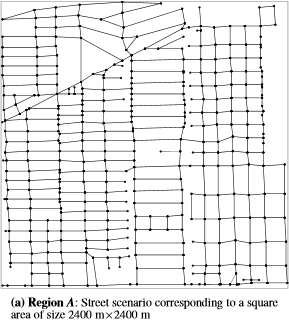
\includegraphics{../images/cityA.png} &
   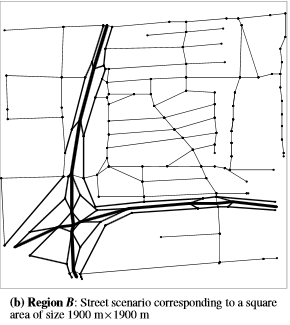
\includegraphics{../images/cityB.png} \\
\end{tabular}



\begin{multicols}{2}
\textit{\textbf{Région A}}
\begin{itemize}
\item Transmission range : 250 meters.
\item 200 nodes.
\item 10\% of the pairs of nodes are incapable to communicate.
\item the connectivity of a network is poor
\item New parameters : Transmission range : 500 meters.
\item 50 nodes.
\item Result : the connectivity fluctuates a lot.
\end{itemize}
\columnbreak
\textit{\textbf{Region B}}
\begin{itemize}
\item Transmission range : 250 meters.
\item 200 nodes.
\item 5\% of the pairs of knots were disconnected.
\item Result: The connectivity is better than in the region A.
\item New parameters : Transmission range : 500 meters.
\item 50 nodes.
\item The area covered in Region B is less than the area covered in Region A.
\item The connectivity corresponding to Region B is better as compared to scenarios corresponding to Region A.
\end{itemize}
\end{multicols}


Another experiment was conducted on the two regions previously mentioned with a routing protocol called DSR. The DSR protocol consists of two mechanisms : Route Discovery and Route Maintenance. According to the article, 
\begin{quotation}
To perform a Route Discovery for a destination node D, a source node S broadcasts a ROUTE REQUEST that gets flooded through the network in a controlled manager. This request is answered by a ROUTE REPLY from either D or some other node that knows a route to D. To reduce frequency and propagation of ROUTE REQUESTs each node aggressively caches source routes that the node learns or overhears.\\
Route Maintenance detects when some link over which a data packet is being transmitted breaks\cite{VehicularAdHocNetworks9}.
\end{quotation}

Simulations were made by using 150 knots with a wireless transmission range of 500m. The communication  pattern  consisted of 10 constant bit rate flows, each sending 4 64 Bytes data packets from the source to the destination.
The evaluation of this protocol is made on 3 properties.
\begin{itemize}
\item Packet Delivery Ratio
\item Packet delivery latency
\item Packet overhead
\end{itemize}

Here are the results obtained with the protocol DSR:\\

\begin{figure}[h]
\center
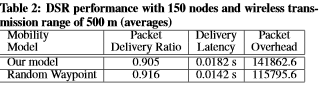
\includegraphics{../images/protocoleDSR.png}
\caption{\label{ProtDSR}DSR Performance}
\end{figure}

We see that the obtained results are very similar in the Waypoint model. The average path length does not differ much.\\
We can conclude that from it the Waypoint model is a very good approximation of the model concerning streets.

Numerous improvements are possible so that the model is realistic :

\begin{itemize}
\item Changing settings depending on the time (lots of car in the morning for example).
\item Possibility of introducing obstacles.
\item Currently, each vehicle moves independently. But in the real life, it has to pay attention on his environment.
\item The model does not take into account the waiting time in the intersections.
\end{itemize}

To conclude, this model uses data of the real life. A called protocol DSR was used to test the model. We were able to notice that the model Waypoint is a good approximation of the model concerning streets.



\subsection{Social Network Theory}

This model bases on the theory of the social networks and on the decisions and the social behavior of the human beings. For example, how the human beings move in a group, and between the groups. A notion of relation between the people is thus identified.\\
In this model, the individuals and the groups of individuals are how considered entities of the first one classes. The second class represents the strength of the social links (probability of collocation).\\

Representation of social networks is made through weighted graphs, by defining the weights associated with each edge of the network to model the strength of direct interactions between individuals. The degree of interaction is a value between 0 and 1. 0 represents no interactions, 1 represents a strong interaction.
The model assumes a level of interaction less than 0.25 represents a social interaction disconnection.\\


\begin{figure}[h]
\center
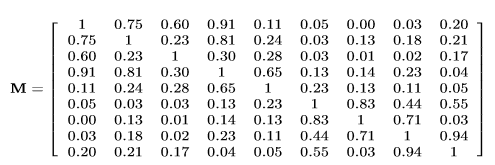
\includegraphics{../images/MatrixInteractionSocialNetwork.png}
\caption{\label{MatricSN}Matrix of interactions between nodes}
\label{MatricSN}
\end{figure}

The objective of this model is to use social relationships between the individuals to define groups of hosts who move together of the scenarios.
The first step is the generation of the social network. It is represented by a matrix of interaction \pageref{MatricSN}.\\

People can be grouped according to their social links or compared with their geographical location. Dynamic mechanisms are present in this model. The people can belong to a group at the moment T, and change group afterward. The notion of distance goes in account into the parameters.\\
A incalculable number of scenarios can be set up. Every groups move with a random speed and every host has a random speed of its own. A host, belonging to a group, moves inside this one. He can reach for example an aim which was fixed to its. Nodes not belonging to any group move randomly.\\

When a knot reached its aim, he has to make a choice:
It is stay in the group to which it is up.
It is chooses to be alone.
This choice is made according to the rate of sociability of the group.The node will join the group which exercises most attraction.\\

Two scenarios are presented for this model. They are characterized by a number of different node and a different number of groups.  The zone of simulation is a square of 1km on 1km, the zone of a group is of 200m. Every group has a speed between 1 and 2 m/s and every node has a speed between 1 and 3 m/s. The first scenario includes 30 computers (representing nodes) consisted in 5 geographically different groups. The second scenario includes 60 computers distributed in 5 groups. In both cases, 80\% of nodes are in a group. Thanks to these scenarios, we can obtain the average degree of connectivity of this model.\\

\begin{tabular}{cc}
   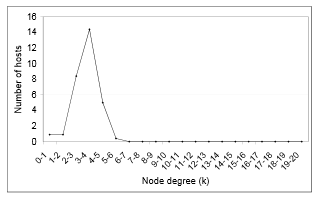
\includegraphics[scale=0.7]{../images/degreeConnectivitySocialNetwork30Nodes.png} &
   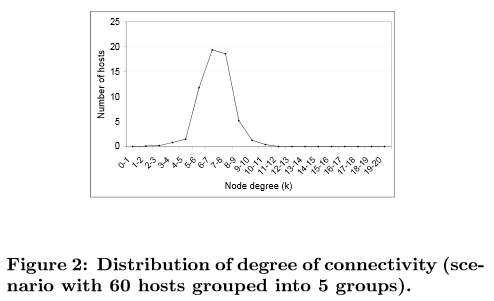
\includegraphics[scale=0.7]{../images/degreeConnectivitySocialNetwork60Nodes.png} \\
\end{tabular}

In conclusion of this model, we can say that generally, the models of existing mobility leans on random movements which are very simplistic and most of the time unrealistic. It is necessary to make models which base themselves on real elements. Here, it is the human socialization which is put forward. But this model can be again improved for example by adding obstacles.




\subsection{Pheromone}

\subsubsection{Description of the model}
This model is inspired by real pheromone. A pheromone is a chemical substance, secreted externally by certain animals, such as insects, affecting the behaviour or physiology of other animals of the same species.\footnote{\url{http://dictionary.reference.com/browse/pheromone?s=t}}
\\
This model use digital Pheromone.This pheromone have 3 properties :

\begin{itemize}
\item  Deposited and withdrawn pheromone from an area. (Information fusion and aggregation).
\item  Evaporated over time. (Forget old information = Truth maintenance).
\item  Propagated from a place to its neighboring places. (Information diffusion and dissemination). 
\end{itemize}

A  digital  pheromone  represents  information  about  the  system. Different  "flavors"  of  pheromones convey different kinds of information.\\ We can have for example, attractive pheromone or repel pheromone. The attractive pheromone will attract other UAVs whereas the repel pheromone will repulse other UAVs.Digital pheromones exist within in an artificial space called a pheromone map.

\subsubsection{Scenario possible}
Pheromone logic  can  be  used  for  several  types  of  surveillance  and target  acquisition  and  tracking scenarios.\\
\begin{itemize}
\item Surveillance and Patrol
\begin{figure}[h]
\center
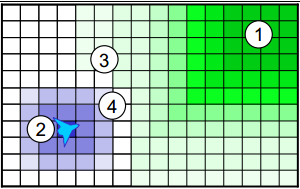
\includegraphics[scale=0.7]{../images/pheromone_surveillance.png}
\caption{\label{surveillance}Attractive and repulsive pheromones for surveillance}
\end{figure}\\\\
In Figure \ref{surveillance}, each step mean :\\
 1. Surveillance area deposits attractive pheromone,\\
 2. UAV deposits repulsive pheromone,\\ 
 3. Pheromone infrastructure propagates both attractive and repulsive pheromone to form gradient,\\
 4. UAV climbs net gradient, withdrawing attractive pheromone.
\item Target Acquisition
\begin{figure}[h]
\center
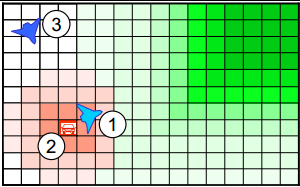
\includegraphics[scale=0.7]{../images/pheromone_target_acquisition.png}
\caption{\label{targetacquisition}Pheromones attracting confirming sensors}
\end{figure}\\\\
In Figure \ref{targetacquisition}, each step mean :\\
1. UAVdet detects target and Red target is created,\\
2. Red target deposits “NeedsID” pheromone, \\
3. UAVid is more attracted to NeedsID pheromone than lawn pheromone and 
climbs gradient to ID target. 
\item Target Tracking
\begin{figure}[h]
\center
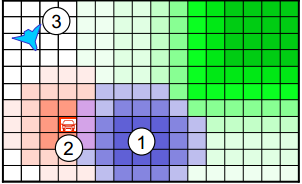
\includegraphics[scale=0.7]{../images/pheromone_tracking.png}
\caption{\label{tracking} Pheromone tracking algorithm}
\end{figure}\\\\
In Figure \ref{tracking}, each step mean :\\
1. UAV acquires target and large Visited pheromone deposit repelling 
other UAVs,\\
2. Red target estimates movement, deposits “Tracking” pheromone that eventually overcomes strength of Visited pheromone, \\
3. Nearby UAV is more attracted to Tracking pheromone than repelled by Visited pheromone and climbs gradient to reacquire the target. 
\end{itemize}
\subsubsection{Real scenario}

We are going to see a real scenario wich demonstrate the use of pheromone model.\\
The demonstration used: 
\begin{itemize}
\item Four robots 
\item A mock urban area  
\item Two UAVs controlled by pheromone technology 
\end{itemize}

\textbf{A CHANGER LE TEXTE CI DESSOU}
The demonstration focused on the swarming algorithms that control and coordinate the behaviors of the heterogeneous mix of vehicles.  
Pheromone  algorithms  controlled  and  coordinated  the  flight  of  the  two  UAVs  as  they  performed 
continuous  surveillance  over  an  urban  area  looking  for  potential  adversaries.  The  two  air  units 
worked together to ensure even, thorough, and continuous coverage of all areas in the surveillance 
region  while  avoiding  any  collisions.  They  also  provided  patrol  coverage  of  a  mock  convoy  as  it 
moved through the area. 
While the UAVs surveyed a broad area over the airfield, the ground robots surveyed and patrolled 
around  some  mock  buildings  set  up  for  the  demo.  During  the  demonstration,  one  of  the  ground 
robots  failed.  The  other  ground  robots  were  able  to  dynamically  readjust  their  patrol  patterns to 
accommodate  the  missing  unit  without  any  intervention  by  the  operator.  This  unplanned  event 
helped to demonstrate the robustness of these algorithms to unexpected events. 
The  demonstration  showed  cooperative  behavior  between  the  air  and  ground  units  when  the 
identity of a potential adversary detected by one of the UAV’s was automatically confirmed by one of 
the ground robots with a special sensor capable of target identification. 
The operator simply gives a high level command to the whole swarm, such as “survey this area and 
track  any  identified  targets”  or  “patrol  around  this  convoy”.  The  robots  autonomously  configured 
themselves to determine which robot would perform what task in order to accomplish the overall 
objective.  



\subsection{Natural Agent}

\subsubsection{Ants}

Le modèle de mobilité des fourmis se base sur le fait que les fourmis construisent des réseaux de sentiers qui relient leurs   nids avec des sources de nourritures disponible.
Chaque fourmi qui se nourrit à le même programme :

\begin{itemize}
\item Elle doit éviter les obstacles.
\item Aller ou elle veut (déplacement aléatoire) tant qu'il n'y a pas de phéromones.
\item Si elle arrive à trouver de la nourriture, elle laisse des phéromones pendant un temps t pour pouvoir indiquer aux autres fourmis l'emplacement de la nourriture.
\item Si la fourmi trouve de la nourriture, elle l'a ramène à son nid.
\end{itemize}

Les fourmis peuvent mourir. Soit elles ne trouvent pas de la nourriture assez rapidement et meurt de faim, soit elles se font tuer par d'autres prédateurs.
Tous les chemins de phéromones conduisent à de la nourriture. Mais les phéromones s'évaporent dans le temps. Le taux de phéromone peut être renforcé si plusieurs fourmis passent par le même chemin.

\textbf{METTRE DES SCHEMA ET a compléter}

\subsubsection{Termites}

\subsubsection{Wasps}

le modèle basé sur les guêpes est composé de plusieurs caractéristiques :
\begin{itemize}
\item un chef qui répartit les différentes guêpes dans différents groupes
\item 
\end{itemize}

\subsection{Birds and Fish}

\subsection{Wolves}
